\documentclass[border=3pt,tikz]{standalone}

\usepackage{tikz}
\usetikzlibrary{decorations.pathmorphing, decorations.pathreplacing, decorations.shapes, }
\usetikzlibrary{angles,quotes} % for pic (angle labels)
%\tikzset{>=latex} % for LaTeX arrow head
\usepackage{amsmath}
\usepackage{graphicx}

\begin{document}

\begin{tikzpicture}

\begin{scope} [yshift=100.0, rotate=30]

\filldraw[black] (2.0,0.0)  circle (0.6pt);
\draw[very thin, ->] (1.0,0.10) arc (30:330:0.05 and 0.20);
\draw[thick] (2.0,0.0) ellipse (0.25 and 1.00);
\draw[thick] ( 1.0,0.0) -- (1.69,0.0);
\draw[color=white,line width=3] ( 2.1,0.0) -- (3.0,0.0);
\draw[thick,->,>=latex] ( 1.81,0.0) -- (3.0,0.0) node [right] {$\boldsymbol{\omega}=\mathbf{u}\dot{\theta}$};

\end{scope}

\begin{scope} [yshift=50.0, rotate=30]
\draw[thick,->,>=latex] ( 1.0,0.0) -- (3.0,0.0) node [right] {$\mathbf{v}=\mathbf{u}\dot{d}$};
\end{scope}

\begin{scope} [ rotate=30]
\draw[thick,decorate,decoration={coil,aspect=0,amplitude=20,segment length=30}] (0,0) -- (3.7,0);
\draw[color=white,line width=3] (-0.1 ,0.0) -- (0.10,0.0);
\draw[thick]                    (-0.4 ,0.0) -- (0.47,0.0);
\draw[color=white,line width=3] ( 0.58,0.0) -- (1.52,0.0);
\draw[thick]                    ( 0.58,0.0) -- (1.52,0.0);
\draw[color=white,line width=3] ( 1.64,0.0) -- (2.57,0.0);
\draw[thick]                    ( 1.64,0.0) -- (2.57,0.0);
\draw[color=white,line width=3] ( 2.69,0.0) -- (4.00,0.0);
\draw[thick,->,>=latex]         ( 2.69,0.0) -- (4.00,0.0) node [right] 
{$\mathbf{t}=\left[\begin{array}{c}
\boldsymbol{\omega}\\
\mathbf{v}
\end{array}\right]$} ;

\draw[very thin] (0.26,0.75) -- (0.26, 1.00);
\draw[very thin] (1.31,0.75) -- (1.31, 1.00);
\draw[very thin, <->, >=latex] (0.25,0.90) -- (1.30, 0.90);
\node[above, rotate=30] at (0.75,0.85) {$d$};

%\draw[color=white,line width=3] (-0.1, 0.10) arc (30:330:0.05 and 0.20);
%\draw[very thin, ->] (-0.1, 0.10) arc (30:330:0.05 and 0.20);
\filldraw[white, line width=2pt] (-0.12,0.1) -- (-0.12,-0.1);
\draw[very thin, ->, rotate=-75] (-0.15, -0.20) arc (225:30:0.20 and 0.05);

\end{scope}

\begin{scope} [xshift=160.0]

% define point
\coordinate (A)  at (4, 3);
\coordinate (O)  at (0, 0);
\coordinate (B)  at (4, 0);
\coordinate (A2) at (2, 1.5);
\coordinate (B2) at (2, 0);

\draw (O) rectangle (A) node[above left] {development of cylinder};
\draw (O) -- (A) ;
% angle  
\draw pic["$\alpha$",draw=black,angle radius=20,angle eccentricity=1.4, <->, >=latex] {angle = B--O--A};

\draw [thick] (O) -- (B2) -- (A2) ;
\draw[very thin] (O)  -- +(0, -1.4) ;
\draw[very thin] (B2) -- +(0, -0.7) ;
\draw[very thin] (A2) -- +(0.7, 0) ;
\draw[very thin] (B)  -- +(0, -1.4) ;
\draw[very thin] (B)  -- +(0.7, 0) ;
\draw[very thin] (A)  -- +(0.7, 0) ;

\draw[very thin, <->, >=latex] (0, -0.55) -- node[above] {$\omega=\dot{\theta}$} (2, -0.55) ;
\draw[very thin, <->, >=latex] (0, -1.25) -- node[above] {$2\pi$} (4, -1.25) ;
\draw[very thin, <->, >=latex] (2.55, 0) -- node[above, rotate=90] {$v=\dot{d}$} (2.55, 1.5) ;
\draw[very thin, <->, >=latex] (4.55, 0) -- node[above, rotate=90] {$d$} (4.55, 3.0) ;

\node[above right] at (-0.3, 4.0) {$\begin{array}{rl}
\text{unit vector :} & \mathbf{u}=\boldsymbol{\omega}/\left\Vert \boldsymbol{\omega}\right\Vert \\
\text{delta angle :} & \theta=\left\Vert \boldsymbol{\omega}\right\Vert \cdot\Delta t\\
\text{angular speed :} & \omega=\left\Vert \boldsymbol{\omega}\right\Vert =\dot{\theta}\\
\text{linear speed :} & v=\left\Vert \mathbf{v}\right\Vert =\dot{d}\\
\text{screw pitch :} & h=v/\omega\\
\text{position vector :} & \boldsymbol{\rho}=\left(\boldsymbol{\omega}\times\mathbf{v}\right)/\omega^{2}\\
\text{twist vector :}&\mathbf{t}=\left[\begin{array}{c}
\boldsymbol{\omega}\\
\mathbf{v}
\end{array}\right]=\omega\left[\begin{array}{c}
\mathbf{u}\\
h\mathbf{u}+\boldsymbol{\rho}\times\mathbf{u}
\end{array}\right]
\end{array}$} ;

\end{scope}


\node[rotate=90] at (12, 1.5) {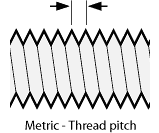
\includegraphics[scale=0.6]{threads-pitch.png}};
\draw[very thin, ->, >=latex] (10.25, 1.5) -- (10.65, 1.5) ;


\end{tikzpicture}

\end{document}
